\chapter{Introduction to Raman spectroscopy}
\label{ch:introduction}

The discovery of the Raman effect is attributed to the physicist Chandrasekhara Venkata Raman, who initially conducted his experiments on the diffusion of light in liquids. In a lecture held in 1930, following the recognition of the Nobel Prize for Physics, he recounts a trip to Europe taken ten years earlier, during which he had a crucial intuition for his work, observing the opalescent blue of the Mediterranean Sea and wondering whether it owed its origin to the interaction between sunlight and the molecules of water. Subsequent experiments led him to conclude that the topic had a meaning that extended far beyond the special purpose for which the work had been undertaken and offered unlimited space for research \cite{raman1930molecular}.

The principle of the Raman effect is based on the assumption that the incident radiation can temporarily perturb the molecule in different ways, in a classical or semi-classical description, and that the scattered light can be observed even at frequencies different from those of the incident radiation. Compared with Rayleigh scattering, this inelastic phenomenon is much weaker in terms of detected intensity, but extremely significant for investigating the physicochemical composition of matter.


\section{Physical description of the Raman effect}
\label{sec:theory_raman_effect}

\subsection{Classical theory: induced dipole and polarizability}
\label{subsec:classical_raman}


The classical theory of Rayleigh and Raman scattering is based on the concept that scattered light is generated by
oscillating electric dipoles induced by the electric field of incident radiation \cite{keresztury2002raman}. 
The electric field of a monochromatic laser beam can be written as
\begin{equation}
    \mathbf{E}(t) = \mathbf{E}_0 \cos(2\pi \nu_0 t),
    \label{eq:incident_field}
\end{equation}
where \(\mathbf{E}_0\) is the field amplitude and \(\nu_0\) is the frequency of oscillation.

When the field interacts with the molecule, the electronic charge distribution is slightly shifted with respect to the nuclei, generating an induced electric dipole, that is, a separation between the centres of positive and negative charge.
The relation between the induced dipole moment vector and the electric field vector to the first order of approximation is 
\begin{equation}
    \boldsymbol{\mu}_{\mathrm{ind}}(t) =
    \boldsymbol{\alpha}\mathbf{E}(t),
    \label{eq:induced_dipole}
\end{equation}
where \(\boldsymbol{\alpha}\) is the polarizability tensor. 
In this view, the polarizability measures how easily the electronic distribution of a molecule, now treated precisely as a polarizable object, can be deformed by the effect of an incident external field.


\subsection{Molecular vibrations and Raman activity}
\label{subsec:molecular_vibrations}

For a simple diatomic molecule, the binding potential energy as a function of internuclear distance is defined by a Morse curve, whose absolute minimum corresponds to the equilibrium geometry. For small oscillations around this equilibrium geometry, the potential can be approximated by a parabola and, to second order, by a harmonic potential. Consequently, the chemical bond is treated as a system of two masses at the ends of a spring that experience a force proportional to their displacement with respect to the equilibrium geometry, as follows from Hooke's law. The frequency of oscillation of the bond is related to its rigidity, as well as its length and the masses of the nuclei. 

For polyatomic molecules, the motion of the nuclei is generally more complex and requires, for an adequate discussion, the introduction of normal modes of oscillation. Each normal mode \(Q_k\) is an independent collective coordinate with its own frequency that describes a pattern of displacements involving multiple atoms.
The normal vibrations are treated as being harmonic, i.e.
\begin{equation}
    Q_k(t) = Q_{k,0}\cos(2\pi \nu_k t),
    \label{eq:normal_coordinate}
\end{equation}
where \(\nu_k\) is the vibrational frequency of the \(k\)-th normal mode.

\begin{figure}[htbp]
    \centering
    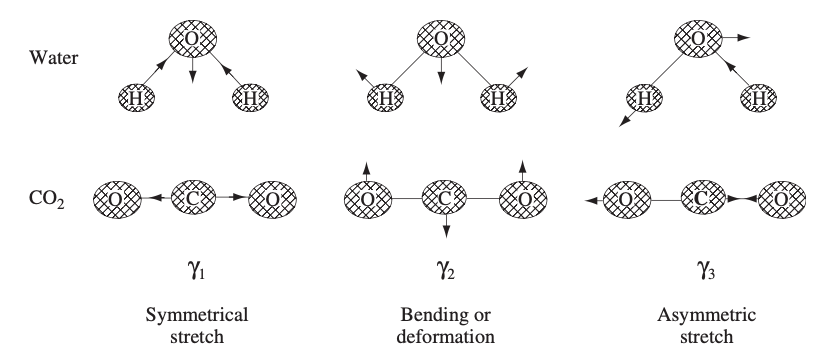
\includegraphics[width=0.80\textwidth]{Images/images_ch_1/normal_modes.png}
    \caption{Examples of normal vibrational modes in simple molecules, such as symmetric stretching, bending or asymmetric stretching \cite{smith2005modernraman}.}
    \label{fig:normal_modes}
\end{figure}

The polarizability of a molecule is a tensor of rank 2 and can be represented by a
two-dimensional (eventually, a \(3 \times 3\)) matrix. 
Expanding the polarizability of the molecule in a Taylor series it gives
\begin{equation}
    \alpha_{ij}(\{Q\}) \simeq
    \left(\alpha_{ij}\right)_0 +
    \sum_k
    \left(\frac{\partial \alpha_{ij}}{\partial Q_k}\right)_0 Q_k  
    \label{eq:polarizability_taylor}
\end{equation}

where \(\alpha_{ij}\) is a component of the polarizability tensor, with
\((\alpha_{ij})_0\) being its value at the equilibrium configuration;
\(Q_k\) is the \(k\)-th normal coordinate associated with vibration frequency
\(\nu_k\); the subscripts \(0\) refer to derivatives taken at the equilibrium configuration.

Inserting equations~\eqref{eq:incident_field} and \eqref{eq:normal_coordinate} into equation~\eqref{eq:induced_dipole} gives, for
the kth vibration,
\begin{equation}
\begin{aligned}
    \mu_{\mathrm{ind},i}(t) \propto {}&
    \underbrace{\sum_j \left(\alpha_{ij}\right)_0 E_{0,j} \cos(2\pi \nu_0 t)}_{\text{Rayleigh}} \\
    &+
    \underbrace{\frac{1}{2}\sum_j
    \left(\frac{\partial \alpha_{ij}}{\partial Q_k}\right)_0
    Q_{k,0}E_{0,j}
    \cos 2\pi(\nu_0-\nu_k)t}_{\text{Stokes}} \\
    &+
    \underbrace{\frac{1}{2}\sum_j
    \left(\frac{\partial \alpha_{ij}}{\partial Q_k}\right)_0
    Q_{k,0}E_{0,j}
    \cos 2\pi(\nu_0+\nu_k)t}_{\text{anti-Stokes}} .
\end{aligned}
\label{eq:induced_dipole_components}
\end{equation}

The three cosine functions having three different arguments in this equation mean that the induced dipole oscillates with three distinct frequencies simultaneously; therefore, it generates radiation at \(\nu_0\) and also at shifts of \(\pm \nu_k\). The first term describes Rayleigh scattering observable at \(\nu_0\), whereas the second and third terms account for Stokes Raman and anti-Stokes Raman scattering at \(\nu_0 - \nu_k\) and \(\nu_0 + \nu_k\), respectively. These so-called beat frequencies are produced when the dipole oscillating at \(\nu_0\) is modulated by the molecular vibration at wavenumber \(\nu_k\). It can be concluded that the classical theory successfully describes the frequency relationships of vibrational Raman scattering. It shows that the Raman shift is independent of
the frequency (wavelength) of the incident radiation \cite{keresztury2002raman}. 

The intensity of Rayleigh scattering
depends on \(\alpha_0\), the polarizability of the molecule at the
equilibrium nuclear configuration, whereas that of Raman
scattering (both Stokes and anti-Stokes) is governed by the derived polarizability tensors, \(\boldsymbol{\alpha}'_k\).

It is clear that the derived tensor serves as the measure of Raman activity: those vibrations for which \(\boldsymbol{\alpha}'_k = 0\) are inactive in Raman scattering, and those normal vibrations for which at least one component of \(\boldsymbol{\alpha}'_k\) differs from zero, i.e.
\begin{equation}
    \left(\alpha'_{ij}\right)_k =
    \left(\frac{\partial \alpha_{ij}}{\partial Q_k}\right)_0
    \neq 0
    \label{eq:raman_activity}
\end{equation}
are Raman active.


\subsection{Quantum interpretation: vibrational levels and virtual states}
\label{subsec:quantum_raman}

To refine the classical description of Raman scattering, it is useful to adopt a semi-classical approach in which the molecule is treated quantum mechanically and the radiation classically as an electromagnetic wave. 

According to the basic principles of quantum mechanics,
the energy associated with electronic, vibrational and rotational degrees of freedom of a molecule can assume only discrete values that correspond to quantised energy levels of the possible stationary states of the molecule. These states are characterised by a specific set of quantum numbers describing
the level of excitation of each motional degree
of freedom, and by a corresponding wavefunction. Each vibrational state is denoted by the quantum numbers \(v = 0, 1, 2, \ldots\).
 
 \begin{figure}[htbp]
    \centering
    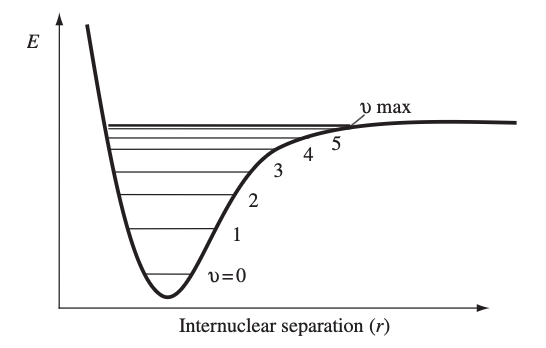
\includegraphics[width=0.60\textwidth]{Images/images_ch_1/molecular_vibrational_states.png}
    \caption{A typical Morse curve for an electronic state showing the vibrational energy levels \cite{smith2005modernraman}.}
    \label{fig:molecular_vibrational_states}
\end{figure}

To describe the interaction of light with matter, electromagnetic radiation is considered as a source of perturbation
of the molecular system.
Radiation is absorbed or emitted by a molecular system as the result
of an upward or downward transition between two energy
levels. Rayleigh and Raman
scattering involve two almost simultaneous transitions proceeding via virtual states in which one photon of the
incident radiation is annihilated and another photon, either
of the same energy (Rayleigh scattering) or of lower energy
(Stokes Raman) or higher energy (anti-Stokes Raman), is
created. The term “virtual state” refers to a very short-lived complex
which does not correspond to an eigenstate of the molecule; it is not stable and exists only during the scattering event.

\begin{figure}[htbp]
    \centering
    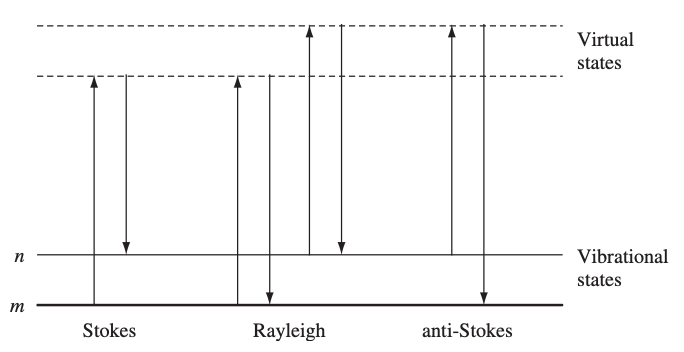
\includegraphics[width=0.65\textwidth]{Images/images_ch_1/stokes_and_anti_stokes.png}
    \caption{Energy-level representation of Rayleigh, Stokes and anti-Stokes scattering \cite{smith2005modernraman}.}
    \label{fig:stokes_anti_stokes}
\end{figure}

\subsection{Selection rules}
\label{subsec:selection_rules}

According to perturbation theory,  the probability for having a transition from an initial stationary state \(\Psi_i\) to a final stationary state \(\Psi_f\), passing through a virtual state, is proportional to the squared modulus of the transition polarizability matrix element \(\alpha_{fi}\). 
\begin{equation}
    P_{i\rightarrow f}^{\mathrm{Raman}} \propto
    \left|\alpha_{fi}\right|^2,
    \qquad
    \alpha_{fi} = \langle \Psi_f|\hat{\alpha}|\Psi_i\rangle .
    \label{eq:raman_transition_probability}
\end{equation}


Each normal mode of oscillation is now modelled as a quantum harmonic oscillator whose vibrational levels are quantised for each kth normal mode. 
Using the first-order expansion of the polarizability tensor (sometimes referred to as the Raman tensor), the probability amplitude will contain a term that couples the initial and final vibrational states, described by their respective quantum numbers  \(v_{i,k}\) and \(v_{f,k}\),  through the coordinate \(Q_k\):
\begin{equation}
    \alpha_{fi}^{\mathrm{Raman}} \propto
    \left(\frac{\partial \alpha_{ij}}{\partial Q_k}\right)_0
    \langle v_{f,k}|Q_k|v_{i,k}\rangle .
    \label{eq:raman_matrix_element}
\end{equation}

A given normal vibration of a molecule may appear
in the Raman spectrum if at least one component of
the polarizability tensor changes during this vibration,
just as in classical theory.
Inserting~\eqref{eq:raman_matrix_element} in~\eqref{eq:raman_transition_probability} , the probability amplitude will contain the matrix element of \(Q_k\) that couples the initial and final vibrational states, described by their respective quantum numbers  \(v_{i,k}\) and \(v_{f,k}\). Only those elements for which the vibrational quantum number changes by unity, \(\Delta v_k=\pm 1\), differ from zero: in this instance a transition is Raman active. As seen previously, the Stokes process corresponds to \(\Delta v_k=+1\), while the anti-Stokes process corresponds to \(\Delta v_k=-1\).

For a molecule with many normal modes, the valid formula is:
\begin{equation}
    \alpha_{fi}^{\mathrm{Raman}} \propto
    \sum_k
    \left(\frac{\partial \alpha_{ij}}{\partial Q_k}\right)_0
    \langle v_{f,k}|Q_k|v_{i,k}\rangle
    \prod_{\ell\neq k}
    \langle v_{f,\ell}|v_{i,\ell}\rangle .
    \label{eq:raman_matrix_element_multimode}
\end{equation}

In this case, all other vibrational quantum numbers remain unchanged (i.e., \(v_{f,\ell} = v_{i,\ell}\) for all \(\ell \neq k\)) since the harmonic oscillator states are orthonormal. 

The classical theory is effective at justifying the position of the transition lines observed in a spectrum, but it is not capable of explaining why, experimentally, anti-Stokes peaks typically exhibit lower intensity compared to Stokes peaks. The reason must be researched in the quantum picture and more specifically discussing the differences in populations of the vibrational energy states. Indeed, at room temperature, the most populated level will be the fundamental state with lower energy, as the Boltzmann distribution proves. This leads to a smaller probability for the anti-Stokes phenomena to occur because it involves molecules that are already excited in a higher vibrational state and are expected to relax to a lower one.
Anti-Stokes peaks approach the height of the Stokes ones only in the case of very low-energy vibration modes, or
when the sample has a high thermal energy. Spectroscopy experiments mainly focus on the Stokes side of the spectra, while the intense Rayleigh component is removed by optical filters.

\subsection{Raman shift and spectral representation}
\label{subsec:raman_shifts}

In practice, Raman spectra are not usually represented as a function of the absolute wavelength of the scattered light. The horizontal axis of the spectrum is the Raman shift, defined as the difference between the wavenumbers of the incident and scattered radiation. For Stokes scattering,
\begin{equation}
    \Delta \tilde{\nu} =
    \tilde{\nu}_0 - \tilde{\nu}_s =
    \frac{1}{\lambda_0} - \frac{1}{\lambda_s},
    \label{eq:raman_shift}
\end{equation}
and it is expressed in \(\mathrm{cm}^{-1}\). 

This convention is useful at a representative level because it highlights the difference in vibrational energy of the molecule following a scattering phenomenon. A certain Raman displacement indicates a specific molecular vibration and does not depend on the laser frequency but only, in fact, on the sample examined.


\section{Spontaneous Raman for biological tissue characterization} 
\label{sec:raman_biological_tissues}

A molecule’s Raman spectrum can be
considered a fingerprint of the molecule itself, identifying it uniquely. Combined with the
recent broad technological advances, this property has established Raman spectroscopy
as a very powerful analytical technique, which is nowadays widely applied across diverse
scientific disciplines.

One spectral interval of particular interest is the \textbf{fingerprint region}, approximately between \(500\) and \(1800~\mathrm{cm}^{-1}\) where one can find peaks associated with a large variety of components, including lipids, proteins, phosphate groups of DNA and RNA,
metabolites, amino acids, Amide I and Amide III bands. The fingerprint region is very
sample specific and particularly suitable to uniquely identify the sample thanks to its
chemical composition.

A second relevant interval is the \textbf{CH region}, around \(2800\)--\(3000~\mathrm{cm}^{-1}\), attributed to
the stretching of CH, CH2, and CH3 chemical bonds, predominantly present in lipids and proteins, from which it takes its name.
Bands in this region are much broader, leading to increased spectral overlap \cite{agrimi2025raman}.

Eventually, the \textbf{silent region}, approximately \(1800\)--\(2800~\mathrm{cm}^{-1}\), is so called because it is mostly empty of contributions from biological molecules.

\begin{figure}[ht]
    \centering
    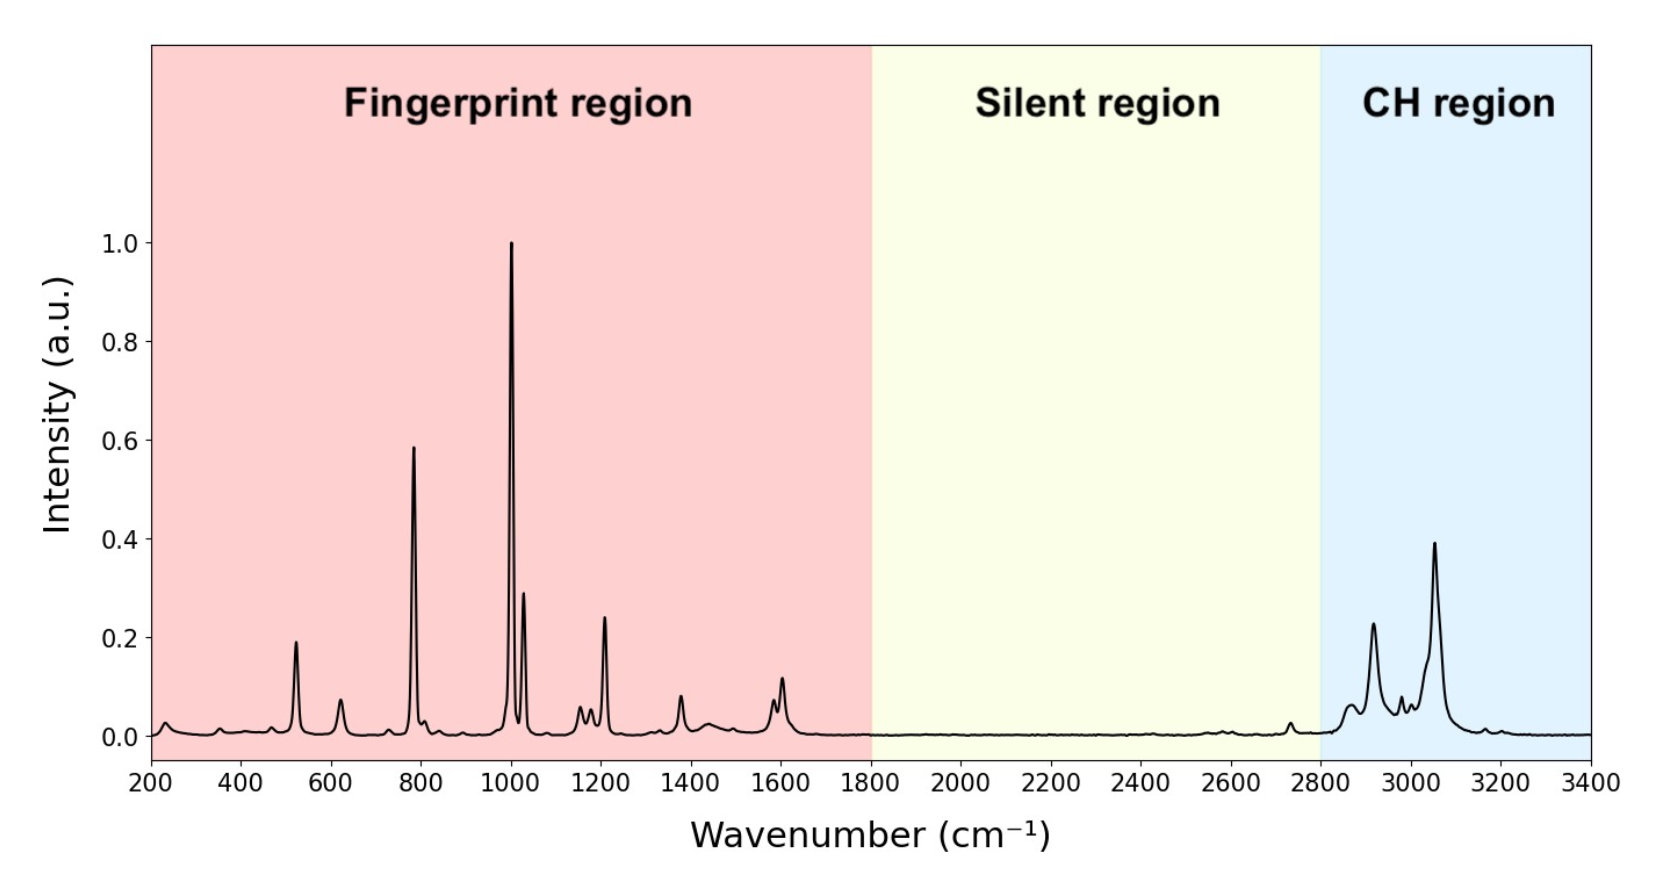
\includegraphics[width=0.65\textwidth]{Images/images_ch_1/regions.png}
    \caption{Representative Raman spectrum highlighting the main spectral regions considered when biological samples are investigated \cite{agrimi2025raman}.}
    \label{fig:raman_spectral_regions}
\end{figure}

In the specific framework of biomedical studies, Raman spectroscopy and microscopy offer many other benefits:
\begin{itemize}
    \item Label-free, allowing the study and false-colour imaging of samples without the need
              for additional substances or markers;

    \item Non-destructive measurements preserve the integrity of the sample
    making it available for further analysis or repeated acquisitions;
    
    \item  Rapid acquisition, especially in the context of intra-operative applications and for
surgical-aid devices;

     \item Minimal sample preparation required.
    \end{itemize}
    
    
The Raman spectrum of a biological sample, its fingerprint as we defined it, is usually difficult to interpret because it results from the overlap of frequency contributions from molecular species with different physical and chemical characteristics. This makes the analysis complex because the relevant information is distributed across the entire spectrum. 

To carry out a classification, given the system's particular heterogeneity, computational methods are extremely useful, as they allow for capturing and interpreting complex patterns distributed across the spectral variables within the intervals described above (fingerprint and CH regions).

   
